\documentclass[11pt,a4paper]{article}

% ---------------------------------------------------------------------------
% Effective approximation, low-intensity bounds, and finite-size effects for
% autocatalytic emergence in reversible polymer networks.
%
% Author metadata: set the three macros below before submission.
% Build: see BUILD.md (pdflatex -> bibtex -> pdflatex -> pdflatex).
% ---------------------------------------------------------------------------
\newcommand{\PaperAuthor}{}
\newcommand{\PaperAffiliation}{}
\newcommand{\PaperDate}{September 2026}

\usepackage[T1]{fontenc}
\usepackage[utf8]{inputenc}
\usepackage{lmodern}
\usepackage{microtype}
\usepackage[a4paper,margin=1.05in]{geometry}
\usepackage{amsmath,amssymb,amsthm,mathtools}
\usepackage{booktabs}
\usepackage{array}
\usepackage{enumitem}
\usepackage{xcolor}
\usepackage{graphicx}
\usepackage{tikz}
\usetikzlibrary{arrows.meta,positioning,calc,decorations.pathreplacing}
\PassOptionsToPackage{hyphens}{url}
\usepackage{url}
\usepackage[colorlinks=true,linkcolor=blue!55!black,citecolor=blue!55!black,urlcolor=blue!55!black]{hyperref}

\setlist{itemsep=2pt,topsep=3pt}
\setlength{\emergencystretch}{1.5em}

\theoremstyle{plain}
\newtheorem{theorem}{Theorem}[section]
\newtheorem{proposition}[theorem]{Proposition}
\newtheorem{lemma}[theorem]{Lemma}
\newtheorem{corollary}[theorem]{Corollary}
\theoremstyle{definition}
\newtheorem{definition}[theorem]{Definition}
\newtheorem{example}[theorem]{Example}
\theoremstyle{remark}
\newtheorem{remark}[theorem]{Remark}

% Breakable typewriter identifiers for Lean names: \lean{Foo.bar_baz}
% (raw underscores permitted; break points after '.' and '_').  Not for captions or math.
\makeatletter
\let\lean@us=_
\let\lean@end\relax
\DeclareRobustCommand{\lean}[1]{\begingroup\ttfamily\lean@scan#1\lean@end}
\def\lean@scan#1{\ifx#1\lean@end\endgroup\else\lean@char{#1}\expandafter\lean@scan\fi}
\def\lean@char#1{\ifx#1\lean@us\char`\_\allowbreak\else\ifx#1.\char`\.\allowbreak\else\ifx#1/\char`\/\allowbreak\else#1\fi\fi\fi}
\makeatother
\newcommand{\leanrefs}[1]{\par\nopagebreak{\small\raggedright\textup{Lean: #1.}\par}}
\newcommand{\conventional}{\par\nopagebreak{\small\raggedright\textup{Conventional proof; not formalised.}\par}}
\newcommand{\mixed}[1]{\par\nopagebreak{\small\raggedright\textup{Conventional proof; Lean-checked components: #1.}\par}}

\newcommand{\Prob}{\mathbb{P}}
\newcommand{\cl}{\mathcal{C}}
\newcommand{\qt}{\mathrm{qt}}
\newcommand{\spc}{\mathrm{sp}}
\newcommand{\eps}{\varepsilon}
\newcommand{\ee}{\mathrm{e}}
\newcommand{\Nat}{\mathbb{N}}
\newcommand{\Real}{\mathbb{R}}
\newcommand{\Rat}{\mathbb{Q}}
\newcommand{\R}{\mathcal{R}}
\newcommand{\word}[1]{\mathtt{#1}}
\DeclareMathOperator{\RAF}{RAF}

\title{Effective approximation, low-intensity bounds,\\ and finite-size effects for autocatalytic emergence\\ in reversible polymer networks}
\author{\PaperAuthor\\ \PaperAffiliation}
\date{\PaperDate}

\begin{document}
\maketitle

\begin{abstract}
The critical-window law for reflexively autocatalytic and food-generated (RAF) sets in the reversible binary-polymer model states that, when the mean number of reactions catalysed per molecule grows like $\lambda n$, the RAF probability converges to $S_\nu(1-\ee^{-\lambda})$, where $S_\nu$ is the probability that ordinary reversible closure of the food set is unbounded in an infinite field of independently open reaction channels. The law is known for the ordered split-position catalogue ($\nu=\spc$) and for the commuting-factor quotient catalogue ($\nu=\qt$). It is an existence theorem: it names the limit but says nothing effective about its value, its shape near zero, or what a finite network actually does. This paper answers those three questions.

First, for both profiles we construct a terminating algorithm which, given rational openness $a$ and rational tolerance $\eps$, returns a rational interval of width below $\eps$ containing $S_\nu(a)$, with an explicit approximation error $1/m+(2^{L+1}-2)(1-a^{L+1})^r$ for a computable seed length $L$ and record index $r$, uniform on every openness interval bounded away from zero. The key estimate is a finite-cap record contraction proved without conditioning on survival and without independence between repair attempts. Second, tracking total word length along productive closure histories replaces a coefficient of order $\binom{J}{r}$ over enormous channel caps by $C_r^\nu\le36^r2^{r(r-1)/2}$, giving $\log S_\nu(a)\le-\log^2(1/a)/(2\log2)+O(\log(1/a))$ and exact certificates such as $S_\nu(10^{-20})<10^{-629}$. Third, at fixed word length $n$ the probability that some singleton RAF exists is exactly $1-(1-p)^{248}$ (split) or $1-(1-p)^{234}$ (quotient), so the finite RAF probability is linear in $p$ at zero while the limiting profile is flatter than every power; we quantify this order-of-limits effect with rational two-sided predictions and two fully explicit examples at $n=16$. We also prove strict monotonicity of the profile, an effective global modulus of continuity, terminating inverse-probability brackets, and non-analyticity at zero. The effective evaluator, its error contract with the finite catalytic model, the settled-history structure and all printed arithmetic are checked in Lean~4; the sharper counting theorem, the singleton law and the regularity results have conventional proofs and are labelled as such.
\end{abstract}

\noindent\textbf{Keywords.} autocatalytic sets; RAF theory; binary polymer model; critical window; computable analysis; certified numerics; productive histories; finite-size effects; formal verification.

\medskip
\noindent\textbf{MSC 2020.} 60K35, 92E20, 05C80, 03D78, 68V20.

\section{Introduction}\label{sec:intro}

A reflexively autocatalytic and food-generated set, or RAF, is a nonempty family of reactions each of whose reactants can be built from a food set using reactions of the family, and each of whose reactions has a catalyst among the molecules so produced. The notion was distilled by Steel~\cite{steel2000emergence} from Kauffman's collectively autocatalytic sets~\cite{kauffman1986autocatalytic,kauffman1993origins} and Eigen's hypercycles~\cite{eigen1971selforganization}, and has been developed into a structural theory with polynomial-time detection algorithms~\cite{hordijk2004detecting,hordijk2012structure,hordijk2015algorithms,steel2019autocatalytic}; see~\cite{hordijk2010autocatalytic,hordijk2017chasing} for surveys. RAF theory is deliberately structural: it asks which reaction families are self-sustaining in principle, and separates that question from kinetics, thermodynamics and molecular inventories. In particular a reaction whose product catalyses it is a singleton RAF, since the catalyst need not be present before the first hypothetical firing. This feature turns out to govern the finite-size behaviour studied below.

The standard random test bed is the binary polymer model~\cite{kauffman1986autocatalytic,steel2000emergence,hordijk2004detecting}: molecules are binary words of length at most $n$, reactions are ligations and their reverse cleavages, the food set consists of the words of length at most two, and each molecule catalyses each reaction independently with a probability chosen so that a molecule catalyses $f_n$ reactions on average. Mossel and Steel~\cite{mossel2005random} showed that $f_n$ growing linearly in $n$ is the relevant scale, and simulations~\cite{hordijk2011required,hordijk2016variable,hordijk2019diversity} display a steep but smooth rise of the RAF probability within a narrow range of $f_n/n$. Two companion manuscripts identified the limit on this scale. For the ordered \emph{split-position} catalogue~\cite{splitwindow2026}, and for the \emph{commuting-factor quotient} catalogue used by the public generator of Varanasi and Korenaga~\cite{varanasi2026emergence,varanasi2026repository,overlapgateway2026,quotientwindow2026}, if $f_n/n\to\lambda>0$ then
\begin{equation}\label{eq:law}
P_n^\nu(p_n)\longrightarrow\Theta_\nu(\lambda)=S_\nu(1-\ee^{-\lambda}),\qquad \nu\in\{\spc,\qt\},
\end{equation}
where $S_\nu(a)$ is the probability that ordinary reversible closure of the food set is unbounded in an infinite field of reaction channels that are independently open with probability $a$. The profile $S_\nu$ is continuous and nondecreasing, $S_\nu(0)=0$, $S_\nu(1)=1$, and $0<S_\nu(a)<1$ on $(0,1)$. Thus the whole linear scale is a nontrivial critical window rather than a threshold.

\subsection*{The questions}
The law~\eqref{eq:law} is an existence theorem. It identifies the limit as a probability in an infinite product space but does not say how to compute $S_\nu(a)$ to a prescribed accuracy, how $S_\nu$ behaves near $a=0$, or how a finite network at moderate $n$ relates to the limit. These are different questions with different answers, and we keep them separate throughout:
\begin{enumerate}[label=(Q\arabic*),leftmargin=3em]
\item \emph{Computability.} Given rational $a$ and rational $\eps>0$, does an explicit algorithm terminate with a rational interval of width below $\eps$ that provably contains $S_\nu(a)$?
\item \emph{Shape.} What can be proved about $S_\nu$ near zero, about strict monotonicity, inverse probabilities and regularity?
\item \emph{Finite size.} What does the finite catalytic model at a given $(n,p)$ actually satisfy, and how does its behaviour near $p=0$ differ from that of the limit?
\end{enumerate}
An answer to one is not an answer to the others. A certified evaluator can exist while being astronomically expensive; a sharp small-openness bound can be proved without any interior evaluation; and a finite network can be governed at small $p$ by a mechanism that is invisible in the limit.

\subsection*{Main results}
Write $M_n=2^{n+1}-2$ for the number of molecules and $R_n^\nu$ for the number of channels of cap $n$; let $p$ be the molecule--channel catalytic probability and $a$ the static channel openness.

\begin{enumerate}[label=\textbf{(\Alph*)},leftmargin=2.6em]
\item \textbf{Effective approximation and a certified evaluator} (Theorems~\ref{thm:approx} and~\ref{thm:algorithm}). For a computable seed length $L=L_\nu(q,m)$ and the caps $D_r=2^r(L+2)-L$,
\[
0\le e^\nu_{D_r}(a)-S_\nu(a)\le\frac1m+(2^{L+1}-2)(1-a^{L+1})^r\qquad(a\in[q,1]),
\]
where $e^\nu_B(a)$ is the finite-cap probability that closure generates a word longer than $B$. Since $e^\nu_B(a)$ is a finite rational computation, this yields a terminating rational enclosure algorithm for $S_\nu$ at every rational $a\in[0,1]$, uniform on $[q,1]$. The heart of the proof is a \emph{record contraction} (Lemma~\ref{lem:contraction}): each escape beyond a cap exposes a fresh record word from which any missing short target can be repaired using at most $\ell+1$ channels of strictly larger product length, and the repair coordinates are disjoint from the exposed prefix. No conditioning on eventual survival and no independence between attempts is used.
\item \textbf{Total-length history bounds} (Theorem~\ref{thm:history}, Corollary~\ref{cor:log}). Along a productive closure history every previously used channel stays settled, so the number of legal next channels is bounded by the square of the number of available types plus the number of cleavage slots, both of which are controlled by the \emph{total word length} of the current set. This gives $S_\nu(a)\le C_r^\nu a^r$ with $C_r^\nu\le36^r2^{r(r-1)/2}$ and hence
\[
\log S_\nu(a)\le-\frac{\log^2(1/a)}{2\log2}+O(\log(1/a)),
\]
replacing the earlier coefficient $\binom{J_r}{r}$ over a channel cap of size $J_r\approx 2^{2^{r+2}}$. Exact certificates such as $S_\nu(10^{-4})<10^{-15}$ and $S_\nu(10^{-20})<10^{-629}$ are kernel-checked.
\item \textbf{Exact singleton law at finite size} (Theorem~\ref{thm:singleton}). For $n\ge4$ the probability that some singleton RAF exists is exactly $1-(1-p)^{A_\nu}$ with $A_{\spc}=248$ and $A_{\qt}=234$, and every RAF without a singleton witness requires at least two positive catalytic coordinates. Consequently $P^\nu_n(p)=A_\nu p+O_n(p^2)$, so the finite network is linear in $p$ at zero while $\Theta_\nu(\lambda)$ is flatter than every power of $\lambda$. The logarithmic rates of the two iterated limits differ (equation~\eqref{eq:exponents}).
\item \textbf{Finite predictions without the approximation cap} (Theorem~\ref{thm:finite}, Section~\ref{sec:examples}). Combining the singleton lower bound with the history bound and the inherited finite catalytic comparison gives
\[
1-(1-p)^{A_\nu}\le P^\nu_n(p)\le\min\{1,\,C_r^\nu(M_np)^r+G_\nu M_{2^{r+1}}p\},
\]
which is evaluable in exact rational arithmetic. At $n=16$ and $\lambda=10^{-4}$ this gives $2.16\cdot10^{-7}<P^{\spc}_{16}<4.57\cdot10^{-5}$ while the limiting profile at the same intensity is below $10^{-15}$.
\item \textbf{Regularity of the profile} (Section~\ref{sec:regularity}). $S_\nu$ is strictly increasing on $[0,1]$ with an explicit finite-forcing lower bound on increments; it has an effective global modulus of continuity including at zero; the inverse map $t\mapsto S_\nu^{-1}(t)$ admits a terminating rational bracketing algorithm; and $S_\nu$ is not real-analytic at zero.
\item \textbf{Formal verification} (Appendix~\ref{app:formal}). The evaluator, the uniform approximation, the record contraction, the seed selector, the finite source contract, the all-powers flatness, the settled-history structure, the generic support union bound and every printed inequality are Lean~4 declarations compiled with warnings promoted to errors and axiom closure $\{$\lean{propext}, \lean{Classical.choice}, \lean{Quot.sound}$\}$. The polymer census behind the sharper coefficient, the singleton semantics, and the regularity results are conventional proofs and are marked as such in the text.
\end{enumerate}

\subsection*{What is new relative to the companions}
We do not reprove the law~\eqref{eq:law}; positivity, continuity, the endpoint values, the supplied-seed mass estimate and the finite catalytic comparison are inherited at their literal source conventions from~\cite{splitwindow2026,quotientwindow2026} and are listed in Section~\ref{sec:inherited}. The companions prove that finite escape probabilities converge to $S_\nu$; they do not give a rate, and their seed lengths are existential. The contribution here is the effective rate, the sharper shape bound, the exact finite-size law, and the regularity results, together with the separation of the three questions above.

\subsection*{Organisation}
Section~\ref{sec:model} fixes both models, the observables and the inherited inputs, and audits the channel counts. Section~\ref{sec:effective} proves the record contraction and the certified evaluator. Section~\ref{sec:history} proves the total-length history bound and its logarithmic corollary. Section~\ref{sec:finite} proves the singleton law and the finite predictions, with two explicit examples. Section~\ref{sec:regularity} proves strict increase, the modulus, inverse brackets and non-analyticity. Section~\ref{sec:discussion} discusses scope and open problems. Appendix~\ref{app:formal} is the concordance between numbered results and Lean declarations.

\section{Models, observables, and inherited inputs}\label{sec:model}

\subsection{Words, channels, closure}
Let $X_n=\bigcup_{\ell=1}^n\{\word0,\word1\}^\ell$ be the nonempty binary words of length at most $n$, $M_n=|X_n|=2^{n+1}-2$, and $F=X_2$ the six food words. A \emph{split channel} is a pair $(w,i)$ with $1\le i<|w|$; it represents the reversible reaction $u+v\rightleftharpoons uv=w$ with $|u|=i$, and its ordered factors are part of its identity. Write $\R_n^{\spc}$ for the split channels of cap $n$; for $n\ge2$,
\begin{equation}\label{eq:splitcount}
R_n^{\spc}=|\R_n^{\spc}|=\sum_{\ell=2}^n(\ell-1)2^\ell=(n-2)2^{n+1}+4.
\end{equation}
The \emph{quotient} model identifies the descriptions $(u,v)$ and $(v,u)$ exactly when $uv=vu$; it never identifies channels with different products. This is the channel catalogue of the generator~\cite{varanasi2026repository} formalised in~\cite{overlapgateway2026,quotientwindow2026}. Write $\R_n^{\qt}$ and $R_n^{\qt}$ for the quotient channels and their number; Lemma~\ref{lem:count} computes $R_n^{\qt}$ exactly. Throughout, $\nu\in\{\spc,\qt\}$ indexes the model, and the inclusions $\R_n^\nu\subseteq\R_{n+1}^\nu$ define the infinite channel set $\R_\infty^\nu$.

For a channel set $A$, the \emph{ordinary reversible closure} $\cl_n(A)$ is the smallest subset of $X_n$ containing $F$ such that whenever the channel of $(u,v)$ lies in $A$: if $u,v\in\cl_n(A)$ then $uv\in\cl_n(A)$, and if $uv\in\cl_n(A)$ then $u,v\in\cl_n(A)$. Availability is set-valued: a factor occurring twice needs one available type, not two copies. The same channel may be used in either direction. There are no concentration, rate, energy or inventory variables. In the infinite channel set the closure $\cl_\infty(A)$ is defined identically without a cap; every membership has a finite derivation.

\subsection{The finite catalytic model}
Let $\xi_{x,r}$, $(x,r)\in X_n\times\R_n^\nu$, be independent Bernoulli variables with parameter $p\in[0,1]$; $\xi_{x,r}=1$ means that $x$ catalyses $r$ in both directions, one mark serving ligation and cleavage. A nonempty $A\subseteq\R_n^\nu$ is a \emph{RAF} if every endpoint of every channel in $A$ lies in $\cl_n(A)$ and every $r\in A$ has some $x\in\cl_n(A)$ with $\xi_{x,r}=1$. This is the closure-based RAF definition of~\cite{hordijk2004detecting,hordijk2011required} for reversible reactions; it coincides with the predicate used in the companions. Food generation is a property of the closure, not of a catalysed order of firing, so a product may serve as the catalyst of its own reaction. Let $P_n^\nu(p)$ be the probability that some RAF exists. Under the \emph{canonical normalisation} $p_n=\lambda n/R_n^\nu$ a molecule catalyses $\lambda n$ channels on average, and $\lambda$ is the dimensionless intensity.

\subsection{The static field and the survival profile}
Independently of catalysis, give each channel $j\in\R_\infty^\nu$ an independent Bernoulli($a$) \emph{open} mark, with product law $\Prob_a$. The \emph{survival profile} is
\begin{equation}\label{eq:survival}
S_\nu(a)=\Prob_a\{\cl_\infty(\text{open channels})\ \text{contains words of arbitrarily large length}\}.
\end{equation}
For a raw length threshold $B\ge2$ let $e^\nu_B(a)$ be the probability that the open closure generates a word longer than $B$. A first crossing of length $B$ is a ligation of two available words of length at most $B$, so the event is determined by the channels of cap $2B$; in particular $e^\nu_B(a)$ is a finite rational computation for rational $a$, and $S_\nu(a)=\lim_{B\to\infty}e^\nu_B(a)$ by monotone continuity. (The formal development indexes escape by $K$ with $B=K+2$; every comparison below is stated in terms of $B$.)

The three parameters used throughout are
\begin{equation}\label{eq:parameters}
p\ \text{(catalytic probability)},\qquad q_k(p)=1-(1-p)^k\ \text{(pool openness)},\qquad a_\lambda=1-\ee^{-\lambda}.
\end{equation}
The pool openness $q_k(p)$ is the probability that at least one of $k$ candidate catalysts marks a given channel; the law~\eqref{eq:law} arises because $q_{M_n}(\lambda n/R_n^\nu)\to a_\lambda$.

\subsection{Gateways and the channel census}
A channel is a \emph{food gateway} if at least one of its sides is wholly contained in $F$; it is a \emph{growth gateway} if in addition its product is not food. Exactly four channels have all endpoints in $F$ (the ligations $\word0+\word0$, $\word0+\word1$, $\word1+\word0$, $\word1+\word1$); we call these \emph{food-only}. Table~\ref{tab:model} collects the counts.

\begin{table}[t]
\centering
\caption{Channel conventions for caps $n\ge4$. A growth gateway produces a nonfood word from two food words; the RAF gateways are all channels with a food side, including the four food-only channels. The last row is proved in Theorem~\ref{thm:singleton}.}
\label{tab:model}
\begin{tabular}{lrr}\toprule
Quantity & Split & Quotient\\\midrule
Food types & 6 & 6\\
Growth gateways $g_\nu$ & 32 & 30\\
RAF gateways $G_\nu$ & 36 & 34\\
Food-only channels & 4 & 4\\
Singleton witness coordinates $A_\nu$ & 248 & 234\\\bottomrule
\end{tabular}
\end{table}

The growth counts need no network enumeration. There are $6^2=36$ ordered ligations of two food words, four of which have a food product, giving $32$ split growth gateways. Quotienting merges the two commuting pairs $(\word0,\word{00}),(\word{00},\word0)$ and $(\word1,\word{11}),(\word{11},\word1)$; no other pair of distinct food words commutes. Adding the four food-only channels gives $G_{\spc}=36$ and $G_{\qt}=34$, the latter being the exact gateway count of~\cite{overlapgateway2026}.

\begin{lemma}[Quotient channel count]\label{lem:count}
Let $\pi_d$ be the number of primitive binary words of length $d$, so that $\pi_d=2^d-\sum_{k\mid d,\,k<d}\pi_k$. Then for $n\ge2$
\begin{equation}\label{eq:deletion}
R_n^{\qt}=R_n^{\spc}-D_n,\qquad D_n=\sum_{d\le n/3}\pi_d\,\#\{(i,j):1\le i<j,\ d(i+j)\le n\}.
\end{equation}
In particular $R_{16}^{\spc}=1\,835\,012$ and $R_{16}^{\qt}=1\,834\,798$.
\end{lemma}
\conventional
\begin{proof}
Two distinct nonempty words $u\ne v$ commute exactly when both are powers of a common primitive word $t$: cancelling the shorter from the longer in $uv=vu$ produces a shorter commuting pair, and iterating terminates at a common root~\cite{lyndon1962equation,lothaire1997combinatorics}. Writing $u=t^i$, $v=t^j$ with $i\ne j$, the split descriptions $(u,v)$ and $(v,u)$ are distinct and merge into one quotient channel; equal exponents give a single description and no merge. Each unordered pair $\{i,j\}$ with $i<j$ and $d(i+j)\le n$ therefore deletes exactly one description per primitive $t$ of length $d$, and $d(i+j)\ge3d$ forces $d\le n/3$. At $n=16$ the contributions for $d=1,\dots,5$ are $112,24,24,24,30$, totalling $214$, and \eqref{eq:splitcount} gives the stated values.
\end{proof}
The formula agrees with literal enumeration for $n\le9$ (Appendix~\ref{app:formal}); the quotient loses only $O(n^22^{n/3})$ of $(n-2)2^{n+1}$ channels, but, as~\cite{quotientwindow2026} shows, the two random experiments are genuinely different and neither profile is a relabelling of the other.

\subsection{Inherited inputs}\label{sec:inherited}
We use the following established results at their literal source conventions~\cite{splitwindow2026,quotientwindow2026}.
\begin{enumerate}[label=(I\arabic*),leftmargin=3em]
\item\label{I:law} $S_\nu(0)=0$, $S_\nu(1)=1$, $0<S_\nu(a)<1$ for $0<a<1$, $S_\nu$ is continuous and nondecreasing, and~\eqref{eq:law} holds for every sequence with $f_n/n\to\lambda>0$.
\item\label{I:seed} \emph{Supplied-seed mass.} Let $C_*=2\cdot7^{64}\cdot81$ be the explicit contour constant of the split source. If $m\ge2$ and $k\ge1$ satisfy
\begin{equation}\label{eq:seedtest}
C_*(1-b^2)^k\bigl(m(m+1)+1\bigr)\le1,
\end{equation}
then, at every static openness $a\ge q$ and in every cap $n$, the closure of $F\cup X_L$ with $L=10k$ occupies fewer than $(m-1)M_n/m$ molecule types with probability at most $1/m$. Here $b=q$ for split channels and $b=q/2$ for quotient channels; the latter uses the at-most-two-to-one channel projection and half-openness domination of~\cite{quotientwindow2026}.
\item\label{I:source} \emph{Finite catalytic comparison.} For $k_{n,m}=(m-1)\lfloor M_n/m\rfloor>6$, near-full static closure at openness $q\le q_{k_{n,m}}(p)$ lower-bounds $P_n^\nu(p)$ up to the mass error of~\ref{I:seed}; and for $n\ge4$, $B\ge2$,
\begin{equation}\label{eq:sourceupper}
P_n^\nu(p)\le e^\nu_B\bigl(q_{M_n}(p)\bigr)+G_\nu M_Bp .
\end{equation}
Every RAF contains a catalysed food gateway, so the RAF event is contained in the gateway event; the second term is a union bound over catalysts of length at most $B$ for the $G_\nu$ food gateways, and it retains food-only RAFs. The split adapter with the exact constant $36$ (rather than the coarse constant $68$ of the earlier source) is compiled in this development.
\end{enumerate}
Condition~\eqref{eq:seedtest} is the contour-ratio form of the supplied-seed estimate: with $z=C_*(1-b^2)^k$ it gives $z/(1-z)\le1/[m(m+1)]$, which is the hypothesis under which the mass theorem delivers error $1/m$. The nontrivial geometric content is inherited; nothing below re-derives it.

\section{Effective finite approximation}\label{sec:effective}

\subsection{An executable seed selector}
For rational $0<q\le1$ and integer $m\ge2$ let $k_\nu(q,m)$ be the least positive integer satisfying~\eqref{eq:seedtest} with $b=q$ ($\nu=\spc$) or $b=q/2$ ($\nu=\qt$), and set $L_\nu(q,m)=10k_\nu(q,m)$. Since $0\le1-b^2<1$ the search terminates by geometric decay, and each test is an exact rational comparison. This replaces the existential seed length of the companions by a computable one. In this section $L=L_\nu(q,m)$.
\leanrefs{\lean{seedTest}, \lean{seedIndex}, \lean{seedIndex_spec}, \lean{rational_deficit_bound}, \lean{selected_contour_deficit}}

\begin{theorem}[Explicit uniform approximation]\label{thm:approx}
Define $D_0=2$ and $D_{r+1}=2D_r+L$, so that $D_r=2^r(L+2)-L$. For every $a\in[q,1]$ and every integer $r\ge0$,
\begin{equation}\label{eq:approx}
0\le e^\nu_{D_r}(a)-S_\nu(a)\le\frac1m+(2^{L+1}-2)(1-a^{L+1})^r .
\end{equation}
\end{theorem}
\leanrefs{\lean{explicit_split_truncation}, \lean{explicit_quotient_truncation}, \lean{split_uniform_approximation}, \lean{quotient_uniform_approximation}}

The proof occupies the rest of this subsection and the next. Fix the model $\nu$ and the openness $a$; all probabilities are with respect to $\Prob_a$ on the infinite static field.

\subsection{Records and fresh repairs}
For a nonempty target word $v$ of length $\ell$ and a threshold $B\ge2$ let $F_B(v)$ be the event that the open closure escapes length $B$ (generates a word longer than $B$) but does not generate $v$ using channels of cap $B$ only.

\begin{lemma}[Bounded record and repair]\label{lem:repair}
On the event of escape beyond $B\ge2$ there is a word $w$ with $B<|w|\le2B$ that is generated using only channels of cap $|w|$. From any such $w$ the target $v$ is generated by cap $|w|+\ell$ as soon as a specified set of at most $\ell+1$ channels is open, and every one of these channels has product length strictly greater than $|w|$.
\end{lemma}
\begin{proof}
Follow a finite derivation witnessing escape and stop at the first step producing a word longer than $B$. Before that step all available words have length at most $B$, and cleavage cannot increase length, so the crossing step is a ligation of two words of length at most $B$ and its product $w$ has $B<|w|\le2B$. The derivation up to and including this step uses only products of length at most $|w|$, so $w$ is generated within its own cap. (Formally one proves by induction on derivations that a generated word is either confined to cap $B$ or the derivation contains such an own-cap record.)

Write $v=v_1\cdots v_\ell$ with each $v_i\in F$. Append the letters successively, $w\to wv_1\to wv_1v_2\to\cdots\to wv$, and finally cleave $wv$ into $w$ and $v$. These are at most $\ell+1$ channel identities (coincidences only reduce the number), each with product length in $(|w|,|w|+\ell]$. In the quotient model, canonicalising a channel preserves its product, so the separation of these repair channels from the cap $|w|$ is preserved; no half-openness comparison is needed for repair marks.
\end{proof}
\leanrefs{\lean{escape_has_bounded_record}, \lean{generated_or_bounded_record}, \lean{finite_record_support}, \lean{quotient_finite_record_support}}

\begin{figure}[t]
\centering
\begin{tikzpicture}[>=Stealth,font=\small,x=1cm,y=1cm]
% axis of word length
\draw[->] (0,0) -- (12.4,0) node[right] {word length};
\foreach \x/\l in {2/{$2$},4/{$B$},7/{$|w|$},8/{$2B$},10.2/{$|w|+\ell$}} {
  \draw (\x,0.08) -- (\x,-0.08); \node[below] at (\x,-0.08) {\l};
}
% exposed prefix region
\fill[black!7] (0.2,0.35) rectangle (7,1.55);
\node[anchor=south west,text width=6.4cm] at (0.25,0.4) {\textit{exposed prefix}: all channels with product length $\le|w|$; the atom fixes their marks and the record $w$};
% record word
\node[draw,thick,rounded corners=2pt,fill=white,inner sep=3pt] (w) at (7,2.4) {record $w$, $B<|w|\le 2B$};
\draw[->,thick] (7,1.6) -- (w.south);
% repair chain
\node[draw,rounded corners=2pt,inner sep=2.5pt] (r1) at (8.2,3.5) {$wv_1$};
\node[draw,rounded corners=2pt,inner sep=2.5pt] (r2) at (9.4,3.5) {$wv_1v_2$};
\node[inner sep=1pt] (dots) at (10.4,3.5) {$\cdots$};
\node[draw,rounded corners=2pt,inner sep=2.5pt] (r3) at (11.4,3.5) {$wv$};
\node[draw,thick,rounded corners=2pt,fill=white,inner sep=3pt] (v) at (11.4,2.1) {$w+v$};
\draw[->] (w.north east) -- (r1.west);
\draw[->] (r1) -- (r2); \draw[->] (r2) -- (dots); \draw[->] (dots) -- (r3);
\draw[->] (r3) -- (v) node[midway,right] {cleave};
\node[anchor=west,text width=4.9cm] at (7.15,1.2) {\textit{repair support}: $\le\ell+1$ fresh channels, products in $(|w|,|w|+\ell]$, disjoint from the prefix};
\draw[decorate,decoration={brace,amplitude=4pt,mirror}] (7.05,-0.55) -- (10.2,-0.55) node[midway,below=4pt] {all repair products live here};
\end{tikzpicture}
\caption{The record-and-repair mechanism of Lemmas~\ref{lem:repair} and~\ref{lem:contraction}. Conditioning on a finite exposed prefix through the first own-cap record $w$ leaves the repair coordinates untouched, so the conditional probability that they are all open is at least $a^{\ell+1}$ regardless of how many earlier attempts failed.}
\label{fig:repair}
\end{figure}

\begin{lemma}[Finite record contraction]\label{lem:contraction}
For $B\ge2$ and every nonempty target $v$ of length $\ell$,
\begin{equation}\label{eq:contraction}
\Prob\bigl(F_{2B+\ell}(v)\bigr)\le(1-a^{\ell+1})\,\Prob\bigl(F_B(v)\bigr).
\end{equation}
\end{lemma}
\begin{proof}
Partition the escape event beyond $B$ according to the first own-cap record length $M>B$ and the complete configuration of the channels with product length at most $M$. These \emph{prefix atoms} are pairwise disjoint and measurable with respect to finitely many coordinates. On each nonempty atom choose a deterministic record carrier $w$ with $|w|=M$; Lemma~\ref{lem:repair} gives $M\le2B$.

Intersect the atom with the event that $v$ is absent from the cap-$B$ closure. This event is also determined by the prefix, so the intersection is a prefix event. The repair support of Lemma~\ref{lem:repair} consists of $s\le\ell+1$ distinct channels with product length above $M$, hence disjoint from the prefix coordinates; conditionally on the prefix its all-open probability is $a^s\ge a^{\ell+1}$. When all repair channels are open, $v$ is generated by cap $M+\ell\le2B+\ell$. Hence on each intersected atom the measure of continued absence of $v$ at cap $2B+\ell$ is at most $(1-a^{\ell+1})$ times the measure of the atom.

Finally $F_{2B+\ell}(v)$ is covered by these continued-absence events: escape beyond $2B+\ell$ implies escape beyond $B$, and absence at the larger cap implies absence at cap $B$. Summing over the disjoint atoms, whose intersections with cap-$B$ absence partition $F_B(v)$, gives~\eqref{eq:contraction}. The argument conditions only on a finite exposed configuration; it neither conditions on eventual survival nor asserts independence between failed attempts.
\end{proof}
\leanrefs{\lean{escaped_missing_contraction}, \lean{quotient_escaped_missing_contraction}, \lean{finite_missing_determined}, \lean{first_record_cap}}

\begin{remark}
The contraction is the effective replacement for the record-word argument of the companions, which proves that unbounded closure eventually generates every fixed word but extracts no rate. The rate $1-a^{\ell+1}$ per doubling of the cap is what makes the seed length below usable in a terminating algorithm. It is also why the approximation is uniform on $[q,1]$: the factor only improves as $a$ increases.
\end{remark}

\subsection{From target repairs to survival}
Iterate~\eqref{eq:contraction} along $d_0=2$, $d_{j+1}=2d_j+\ell$; after $r$ steps the residual probability of escaping $d_r$ while missing $v$ at cap $d_r$ is at most $(1-a^{\ell+1})^r$. If $\ell\le L$ then $d_r\le D_r$ and $1-a^{\ell+1}\le1-a^{L+1}$. A union bound over the $M_L=2^{L+1}-2$ words of $X_L$ gives
\begin{equation}\label{eq:escape-seed}
\Prob\bigl(\text{escape beyond }D_r\text{ and fail to acquire }X_L\text{ by cap }D_r\bigr)\le M_L(1-a^{L+1})^r .
\end{equation}
No independence between the repairs of different targets is used.
\leanrefs{\lean{repeated_record_failure}, \lean{common_cap_target_failure}, \lean{finite_seed_failure}, \lean{exposure_budget}}

Let $H_L$ be the event that all of $X_L$ is acquired in the infinite field. The supplied-seed estimate~\ref{I:seed} gives
\begin{equation}\label{eq:seed-survival}
\Prob(H_L)\le S_\nu(a)+1/m .
\end{equation}
Here is the finite-to-infinite step, which is where an effective seed replaces an existential one. Fix a length $A$. On the event that the food closure stays inside $X_A$ it has at most $M_A$ types. If $X_L$ has been acquired by cap $n$, the closure of $F\cup X_L$ in cap $n$ is contained in the food closure. For all large $n$, $(m-1)M_n>mM_A$, so acquisition together with boundedness forces the supplied-seed mass failure, whose probability is at most $1/m$. Letting $n\to\infty$ exhausts the finite witnesses of acquisition and letting $A\to\infty$ exhausts bounded closure. Hence $\Prob(H_L\cap\{\text{bounded}\})\le1/m$, which is~\eqref{eq:seed-survival}. Both events live in the same field.
\leanrefs{\lean{effective_seed_probability_le_survival}, \lean{effective_quotient_seed_survival}}

\begin{proof}[Proof of Theorem~\ref{thm:approx}]
Split the event of escape beyond $D_r$ according to whether $X_L$ has been acquired by cap $D_r$. The failure branch has probability at most~\eqref{eq:escape-seed}; the success branch is contained in $H_L$ and has probability at most~\eqref{eq:seed-survival}. Survival implies escape beyond every cap, which is the lower inequality. The closed form $D_r+L=2^r(L+2)$ follows by induction.
\end{proof}

\subsection{The certified evaluator}
\begin{theorem}[Certified rational evaluation]\label{thm:algorithm}
For either model there is an explicit terminating algorithm which, given rational $a\in[0,1]$ and rational $\eps>0$, returns a rational interval of width less than $\eps$ containing $S_\nu(a)$. The escape cap computed for a positive rational lower endpoint $q$ controls every real openness $a\ge q$ with the same error budget.
\end{theorem}
\leanrefs{\lean{splitCertifiedInterval_correct}, \lean{quotientCertifiedInterval_correct}, \lean{splitTotalInterval_correct}, \lean{quotientTotalInterval_correct}, \lean{splitEscapeEval_correct}, \lean{quotientEscapeEval_correct}, \lean{recordIndex_error}}
\begin{proof}
At $a=0$ return $[0,0]$, using $S_\nu(0)=0$. Otherwise put $m=\lceil4/\eps\rceil+2$, so $1/m\le\eps/4$; compute $L=L_\nu(a,m)$; and let $r$ be the least positive integer with
\begin{equation}\label{eq:rtest}
2^{L+1}(1-a^{L+1})^r\le\eps/4 .
\end{equation}
This is an exact rational test that terminates by geometric decay, the case $a=1$ being immediate. Now evaluate $e=e^\nu_{D_r}(a)$ exactly: the event is determined by the finitely many channels of cap $2D_r$; for each Boolean configuration iterate the one-step closure operator $M_{2D_r}$ times, which computes the full finite closure since each round either adds a type or is stable; sum the weights $a^s(1-a)^{J-s}$ over the configurations witnessing escape, where $J$ is the channel cardinality and $s$ the number of open channels. By Theorem~\ref{thm:approx}, $[e-\eps/2,e]$ contains $S_\nu(a)$ and has width $\eps/2<\eps$; it may be intersected with $[0,1]$ without losing containment.

For uniformity compute $L$, $r$ and $D_r$ at the lower endpoint $q$. The seed bound~\ref{I:seed} is uniform for $a\ge q$, and $(1-a^{L+1})^r\le(1-q^{L+1})^r$, so the same budget applies. Every search in this construction terminates by a proof, and the finite-event semantics are proved rather than assumed; no approximation oracle enters.
\end{proof}

\begin{remark}[Cost]\label{rem:cost}
Theorem~\ref{thm:algorithm} is a computability statement in the sense of computable analysis~\cite{weihrauch2000computable}, not a practical interior algorithm. At $m=100$ and $q=1/2$ the selected seed lengths are $L=4830$ (split) and $L=21520$ (quotient); already in the split case a repair error of $0.01$ requires a record index with $\log_2r\approx4843$, after which the recurrence $D_{r+1}=2D_r+L$ and the enumeration of channel fields in cap $2D_r$ are applied. These are the costs of the \emph{proof}, not estimates of $S_\nu$. Section~\ref{sec:history} obtains useful bounds without constructing any such cap, and Section~\ref{sec:finite} obtains useful finite predictions without it.
\end{remark}

\section{Total-length history bounds}\label{sec:history}

A \emph{productive history} is an ordered list of distinct channels $r_1,\dots,r_k$, starting from $C_0=F$, such that each $r_{j+1}$ is enabled by the current available set $C_j$ (one side of the channel is available) and adds at least one new type; $C_{j+1}$ is $C_j$ together with all endpoints of $r_{j+1}$. Productive histories are the combinatorial skeleton of closure. The following structural lemma is what makes counting them efficient.

\begin{lemma}[Settled channels and finite histories]\label{lem:settled}
After every productive step all endpoints of every previously used channel belong to the current set, and the current set is exactly the full closure of $F$ under the channels used so far. If the open closure reaches a word longer than $2^{r+1}$, then there is a productive history of $r$ distinct open channels; in particular survival supplies such a history for every $r$.
\end{lemma}
\begin{proof}
The first assertion holds initially and persists: after firing an enabled channel its previously missing endpoints are available, so it too is settled, and settled channels stay settled when types are added. The new set is closed under every channel used so far, is reachable from $F$ by those channels, and contains $F$; hence it is their full closure. In particular adjoining a new channel causes no further cascade through earlier channels.

In $j$ steps the maximum word length is at most $2^{j+1}$, since a ligation at most doubles length and a cleavage does not increase it. If the current set omits a target that is reachable using all open channels, then some open channel is productive on the current set: otherwise the set is closed under all open channels and contains $F$, hence contains the target. A previously used channel cannot be productive because it is settled, so the productive channel is new. Repeat $r$ times; the length bound prevents reaching the long target early. In the infinite field the target has a finite derivation, so the whole argument takes place in a finite cap; no infinite scheduling is needed.
\end{proof}
\leanrefs{\lean{settled_insert_closure}, \lean{productive_history_settled}, \lean{productive_history_ordered}, \lean{split_long_target_history}, \lean{quotient_long_target_history}, \lean{split_unbounded_histories}, \lean{quotient_unbounded_histories}, \lean{publication_history_resolution}}

\begin{lemma}[Length and cleavage-slot budgets]\label{lem:budget}
For a productive history let $T_j=\sum_{w\in C_j}|w|$ and $Q_j=\sum_{w\in C_j}(|w|-1)$. Then for all $j\ge0$
\begin{equation}\label{eq:budgets}
|C_j|\le6+2j,\qquad\max_{w\in C_j}|w|\le2^{j+1},\qquad T_j\le2^{j+2}+6,\qquad Q_j\le4\cdot2^j-j .
\end{equation}
\end{lemma}
\begin{proof}
Initially $(|C_0|,T_0,Q_0)=(6,10,4)$ and each step adds at most two types. A productive ligation adds one word of length at most $2^{j+2}$, increasing $T$ by at most $2^{j+2}$ and $Q$ by at most $2^{j+2}-1$. A productive cleavage of an available product $w$ adds its factors; their total length is $|w|\le2^{j+1}$ whether or not one factor was already present or the factors coincide, and at least one factor is new, so $T$ increases by at most $|w|$ and $Q$ by at most $|w|-1$. Summing $T_{j+1}-T_j\le2^{j+2}$ and $Q_{j+1}-Q_j\le2^{j+2}-1$ gives the last two bounds.
\end{proof}
\conventional
The point of tracking $T_j$ and $Q_j$ as \emph{sums} rather than as (maximum length)$\times$(cardinality) is the quantitative gain: the number of cleavage candidates is the number of split positions in available words, which is $Q_j$, not $|C_j|\cdot2^{j+1}$. Neither quantity is a physical mass; both count word types.

Set $C_0^\nu=1$ and, for $r\ge1$,
\begin{equation}\label{eq:Cr}
b_j=(6+2j)^2+4\cdot2^j-j\quad(j\ge1),\qquad C_r^\nu=g_\nu\prod_{j=1}^{r-1}b_j ,
\end{equation}
so that $C_1^\nu=g_\nu$, $C_2^{\spc}=32\cdot71=2272$ and $C_2^{\qt}=30\cdot71=2130$.

\begin{theorem}[History upper bound]\label{thm:history}
For $a\in[0,1]$, $r\ge0$ and either model,
\begin{equation}\label{eq:history}
S_\nu(a)\le e^\nu_{2^{r+1}}(a)\le\min\{1,\,C_r^\nu a^r\}\le\min\{1,\,(36a)^r2^{r(r-1)/2}\}.
\end{equation}
The middle inequality also holds when the channels are independently open with nonidentical probabilities all bounded by $a$.
\end{theorem}
\begin{proof}
From $C_0=F$ exactly the $g_\nu$ growth gateways are productive: food-only channels add nothing, and a cleavage of a food word yields food. After $j\ge1$ steps, at most $|C_j|^2$ ordered factor pairs can be ligated and at most $Q_j$ (product, split position) pairs can be cleaved; discarding non-productive candidates or identifying quotient duplicates cannot increase the count. Lemma~\ref{lem:budget} bounds the total by $b_j$. Hence there are at most $C_r^\nu$ legal ordered histories of length $r$, and the family is finite because each prefix has finite branching and the length bound confines every endpoint to a finite word universe.

By Lemma~\ref{lem:settled}, escape beyond $2^{r+1}$ is covered by the events that all $r$ channels of some history in this deterministic family are open. A fixed history has $r$ distinct channel identities, so its cylinder event has probability $a^r$; for heterogeneous independent marks it is the product of the $r$ marginals, at most $a^r$. The union bound over the family gives the middle inequality. The histories are enumerated before probabilities are assigned; no claim is made that an adaptively chosen next mark is an unconditioned Bernoulli variable.

For the closed envelope, $(6+2j)^2\le32\cdot2^j$ for $j\ge1$ (equality at $j=1$, and $(8+2j)^2\le2(6+2j)^2$ for $j\ge1$ by expanding), so $b_j\le36\cdot2^j$ and $g_\nu\le36$; multiplying gives $C_r^\nu\le36^r2^{r(r-1)/2}$. The case $r=0$ is the trivial bound one.
\end{proof}
\mixed{the generic union-bound step \lean{history_support_union_bound}, the coefficient envelope \lean{historyBudget_envelope}, and the history extraction of Lemma~\ref{lem:settled}; the polymer census bounding the branching by $b_j$ is conventional}

\begin{remark}[Comparison with the sparse-support bound]\label{rem:sparse}
The companions' all-powers flatness rests on the observation that $r$ open channels confine closure to length $2^{r+1}$, so escape requires $r$ open channels among the $J_r=R^{\spc}_{2(2^{r+1}+2)}$ channels of the witness cap, giving $S_\nu(a)\le\binom{J_r}{r}a^r$. This is valid, Lean-checked, and numerically useless beyond very small $r$: at $r=2$ the coefficient is $\binom{J_2}{2}=712\,483\,666\,919\,430$ against $C_2^{\spc}=2272$, and $J_r$ grows like $2^{2^{r+2}}$. The settled-history structure removes the dependence on the cap entirely. Figure~\ref{fig:bounds} compares the two envelopes.
\end{remark}
\leanrefs{\lean{split_sparse_real}, \lean{quotient_sparse_real}, \lean{split_second_coefficient}, \lean{worked_low_openness_bound}}

\begin{corollary}[Logarithmic shape and flatness]\label{cor:log}
Put $x=\log(1/a)$, $h=\log2$ and $y=x-\log36+h/2$. For $0<a<1$ with $y\ge0$,
\begin{equation}\label{eq:logshape}
\log S_\nu(a)\le-\frac{y^2}{2h}+\frac h8=-\frac{\log^2(1/a)}{2\log2}+O(\log(1/a)).
\end{equation}
In particular $S_\nu(a)=o(a^d)$ for every fixed $d$, and $\Theta_\nu(\lambda)=S_\nu(a_\lambda)=o(\lambda^d)$ as $\lambda\downarrow0$, with the same logarithmic expansion in $\log(1/\lambda)$.
\end{corollary}
\begin{proof}
The logarithm of the last expression in~\eqref{eq:history} is $hr^2/2-yr$. Choose $r$ to be a nearest nonnegative integer to $y/h$; then $|r-y/h|\le1/2$ and completing the square gives~\eqref{eq:logshape}. The logarithm is defined because $S_\nu(a)>0$ by~\ref{I:law}. Flatness follows directly from~\eqref{eq:history} with $r=d+1$. Since $0<a_\lambda\le\lambda$, the intensity statement follows from the same fixed-power bound, and $\log(1/a_\lambda)=\log(1/\lambda)+O(\lambda)$ transfers the expansion.
\end{proof}
\mixed{the all-powers flatness statements \lean{split_low_openness_flatness}, \lean{quotient_low_openness_flatness}, \lean{split_low_intensity_flatness}, \lean{quotient_low_intensity_flatness} (via the sparse coefficient); the logarithmic optimisation is conventional}

The estimate~\eqref{eq:logshape} is one-sided. It is not an asymptotic equivalence and no optimality is claimed for the coefficient $1/(2\log2)$; matching lower bounds are an open problem (Section~\ref{sec:discussion}).

\begin{figure}[t]
\centering
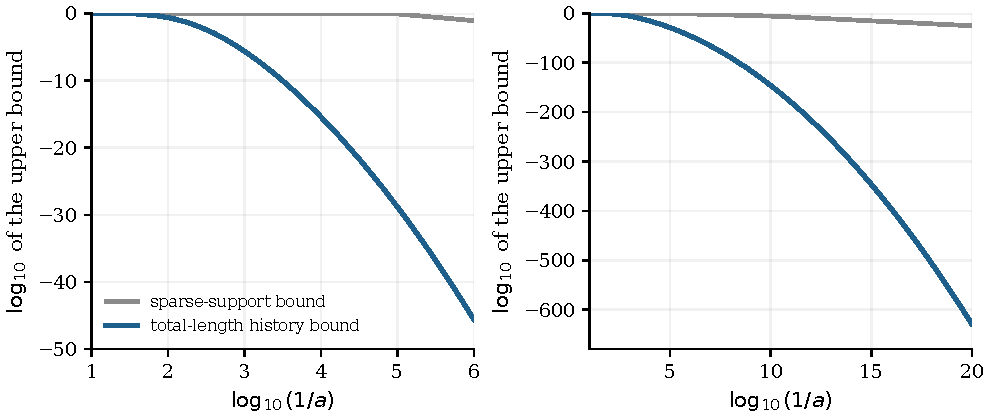
\includegraphics[width=\linewidth]{figures/history_bounds.pdf}
\caption{Upper bounds on the split profile, not a plot of $S_{\spc}$. Grey: the sparse-support envelope $\min_{1\le r\le10}\binom{J_r}{r}a^r$ of Remark~\ref{rem:sparse}. Blue: the total-length history envelope $\min_{0\le r\le80}C_r^{\spc}a^r$ of Theorem~\ref{thm:history}. Both are clipped at one; the left panel enlarges the moderate range. Logarithms are floating-point renderings; the certificates in Table~\ref{tab:small} are exact.}
\label{fig:bounds}
\end{figure}

\begin{table}[t]
\centering
\caption{Exact history-product certificates $C_r^{\spc}a^r<10^{-t}$, valid for both models since $C_r^{\qt}\le C_r^{\spc}$. The indices $r$ need not be optimal. The integer/rational comparisons are kernel-checked; their probabilistic meaning uses Theorem~\ref{thm:history}.}
\label{tab:small}
\begin{tabular}{cccc}\toprule
Openness $a$ & History length $r$ & $\log_{10}C_r^{\spc}$ (approx.) & Certified consequence\\\midrule
$10^{-3}$ & 8 & 18.354 & $S_\nu(a)<10^{-5}$\\
$10^{-4}$ & 12 & 32.578 & $S_\nu(a)<10^{-15}$\\
$10^{-6}$ & 18 & 62.431 & $S_\nu(a)<10^{-45}$\\
$10^{-20}$ & 65 & 670.814 & $S_\nu(a)<10^{-629}$\\\bottomrule
\end{tabular}
\end{table}
\leanrefs{\lean{history_certificate_003}, \lean{history_certificate_004}, \lean{history_certificate_006}, \lean{history_certificate_020}, \lean{publication_small_openness_arithmetic}}

\begin{proposition}[Independence is essential]\label{prop:correlated}
Let one Bernoulli($a$) variable open every channel simultaneously. Then every channel is open with marginal probability $a$, yet the survival probability equals $a$ exactly.
\end{proposition}
\begin{proof}
When all channels are open the closure generates every word; when all are closed it stays at $F$.
\end{proof}
\conventional
Marginal openness bounds alone therefore cannot imply any all-powers estimate. The heterogeneous independent extension in Theorem~\ref{thm:history} accommodates missing or less probable channels; correlated catalytic mechanisms would need a separate dependence theorem.

\section{Finite-network contributions and predictions}\label{sec:finite}

\subsection{Singleton RAFs and the first-order law}
Write $Q_n^\nu=M_nR_n^\nu$ for the number of catalytic coordinates of cap $n$.

\begin{theorem}[Exact singleton contribution]\label{thm:singleton}
For $n\ge4$ let $A_{\spc}=248$ and $A_{\qt}=234$. Then
\begin{align}
\Prob_p(\text{some singleton RAF exists})&=1-(1-p)^{A_\nu},\label{eq:singleton}\\
0\le P^\nu_n(p)-\bigl[1-(1-p)^{A_\nu}\bigr]&\le\binom{Q_n^\nu}{2}p^2.\label{eq:firstordererror}
\end{align}
Consequently, for each fixed $n\ge4$,
\begin{equation}\label{eq:firstorder}
P^\nu_n(p)=A_\nu p+O_n(p^2),\qquad P^\nu_n(\lambda n/R_n^\nu)=\frac{A_\nu n}{R_n^\nu}\,\lambda+O_n(\lambda^2).
\end{equation}
\end{theorem}
\begin{proof}
A single channel $\{r\}$ is food-generated exactly when $r$ is a food gateway: if neither side of $r$ lies in $F$ the channel can never fire alone, so $\cl_n(\{r\})=F$ contains no endpoint of $r$ outside $F$. A food-only channel has $\cl_n(\{r\})=F$, so it has six candidate catalysts. A growth gateway $r$ with product $w\notin F$ has $\cl_n(\{r\})=F\cup\{w\}$, so it has seven candidate catalysts, the product $w$ among them; the structural RAF definition allows a product to catalyse its own reaction, and a kinetic start-up restriction would define a different model. Hence the set of single catalytic coordinates $(x,r)$ certifying a singleton RAF has exactly $4\cdot6+7g_\nu=A_\nu$ elements. The coordinate includes the channel identity, so witness sets of different channels are disjoint even when they share a catalyst molecule, and independence gives~\eqref{eq:singleton}.

If at most one coordinate is positive and a RAF $A$ exists, every channel of $A$ must be catalysed through that one coordinate, so $A$ is a singleton. Hence the event that a RAF exists but no singleton witness is present is contained in the event that at least two coordinates are positive, whose probability is at most $\binom{Q_n^\nu}{2}p^2$ by the union bound over pairs. This gives~\eqref{eq:firstordererror}, and expanding the polynomial $1-(1-p)^{A_\nu}$ at $p=0$ gives~\eqref{eq:firstorder}.
\end{proof}
\conventional
The census $A_{\spc}=248$, $A_{\qt}=234$ is confirmed by literal enumeration at $n=4$ (Appendix~\ref{app:formal}); the universal statement for all $n\ge4$ is the argument above.

\begin{corollary}[Order of limits]\label{cor:exponents}
For each fixed $n\ge4$,
\begin{equation}\label{eq:exponents}
\lim_{\lambda\downarrow0}\frac{\log P^\nu_n(\lambda n/R_n^\nu)}{\log\lambda}=1,\qquad
\lim_{\lambda\downarrow0}\frac{\log\Theta_\nu(\lambda)}{\log\lambda}=+\infty .
\end{equation}
Moreover, conditional on the food-inclusive gateway event (some food gateway catalysed by some molecule), whose probability is $1-(1-p)^{G_\nu M_n}$, the RAF probability at fixed $n$ tends to $A_\nu/(G_\nu M_n)$ as $p\downarrow0$, whereas the corresponding limiting ratio $\Theta_\nu(\lambda)/(1-(1-a_\lambda)^{G_\nu})$ is still $o(\lambda^d)$ for every $d$.
\end{corollary}
\begin{proof}
The first logarithm is $\log\lambda$ plus a constant plus $o(1)$ by~\eqref{eq:firstorder}. For the second, Theorem~\ref{thm:history} with $a_\lambda\le\lambda$ gives $\log\Theta_\nu(\lambda)\le\log C_r^\nu+r\log\lambda$ for every $r$, and positivity makes the quotient well defined; dividing by $\log\lambda<0$ gives $\liminf\ge r$ for every $r$. Every RAF contains a catalysed food gateway (Section~\ref{sec:inherited}), so the conditional statement follows from~\eqref{eq:firstorder}; in the limit the denominator is at least $a_\lambda$, so at most one power is lost.
\end{proof}
\mixed{\lean{conditional_intensity_flatness}, \lean{split_conditional_intensity_flatness}, \lean{quotient_conditional_intensity_flatness}; the finite-$n$ limits are conventional}

The unscaled probabilities vanish in both iterated limits; what differs is the rate. This is the precise sense in which a fixed finite network and the critical-window limit disagree at small intensity, and it is entirely due to singleton witnesses, which have no analogue in the infinite static field.

\subsection{A finite error contract}\label{sec:contract}
The effective evaluator also calibrates a finite catalytic source, even in regimes where the history bound is not small. Let $h^\nu_{n,L}(q)$ be the static probability that the food closure in cap $n$ contains $X_L$, with $L\le n$. Choose $m\ge2$, $k_{n,m}>6$, rational $0<q\le q_{k_{n,m}}(p)$, and the computed seed length $L=L_\nu(q,m)$. In the same field, acquisition of $X_L$ and success of supplied-seed mass imply near-full food closure, so~\ref{I:source} gives
\begin{equation}\label{eq:sourcecontract}
h^\nu_{n,L}(q)-\frac1m\ \le\ P^\nu_n(p)\ \le\ e^\nu_B\bigl(q_{M_n}(p)\bigr)+G_\nu M_Bp .
\end{equation}
Both finite probabilities are exactly rational for rational inputs. If $[l_P,u_P]$ is such a source enclosure and $[l_S,u_S]$ a profile enclosure from Theorem~\ref{thm:algorithm}, then
\begin{equation}\label{eq:comparison}
|P^\nu_n(p)-S_\nu(a)|\le\max\{u_P-l_S,\,u_S-l_P\}.
\end{equation}
\leanrefs{\lean{splitSourceInterval_correct}, \lean{quotientSourceInterval_correct}, \lean{interval_comparison_error}, \lean{split_source_profile_error}, \lean{quotient_source_profile_error}, \lean{canonical_raf_le_finite_escape_36}}
This contract retains the actual input $p$; it is not a cap-only convergence rate for an unspecified sequence $f_n/n\to\lambda$, and cannot be, since a convergent sequence may sit one unit from its limit at any prescribed finite index.

\begin{theorem}[History-based finite prediction]\label{thm:finite}
Let $n\ge4$, $r\ge1$ and $B=2^{r+1}$ with $2B\le n$. For every legal catalytic probability $p$,
\begin{equation}\label{eq:finitehistory}
1-(1-p)^{A_\nu}\ \le\ P^\nu_n(p)\ \le\ \min\{1,\,C_r^\nu(M_np)^r+G_\nu M_Bp\}.
\end{equation}
\end{theorem}
\begin{proof}
The lower bound is~\eqref{eq:singleton}. For the upper bound apply the finite-escape form $e^\nu_{2^{r+1}}(a)\le C_r^\nu a^r$ of Theorem~\ref{thm:history} inside~\eqref{eq:sourceupper} with $a=q_{M_n}(p)\le M_np$, the last inequality being the union bound over catalyst opportunities. The estimate remains valid when $M_np>1$, though clipping at one may then be uninformative. The cap restriction $2B\le n$ keeps the escape event inside the ambient word universe and suffices for the examples.
\end{proof}
\conventional
Increasing $r$ improves the history term at small openness but lets $M_{2^{r+1}}p$ grow doubly exponentially; a useful choice controls the sum.

\subsection{Two exact examples at cap sixteen}\label{sec:examples}
Take $n=16$, $\lambda=10^{-4}$, $r=2$ and $B=8$, so $M_n=131\,070$, $M_B=510$, $2B=n$, $C_2^{\spc}=2272$ and $C_2^{\qt}=2130$; the channel counts are those of Lemma~\ref{lem:count}. Each model uses its own normalisation $p=16/(10^4R_{16}^\nu)$, that is $p=1/1\,146\,882\,500$ (split) and $p=1/1\,146\,748\,750$ (quotient). Bonferroni's inequality gives the computable lower bound $\Lambda_\nu=A_\nu p-\binom{A_\nu}{2}p^2\le1-(1-p)^{A_\nu}$; write $U_{\mathrm{hist}}=C_2^\nu(M_np)^2$ and $U_{\mathrm{short}}=G_\nu M_Bp$. Table~\ref{tab:finite} displays the three terms.

\begin{table}[t]
\centering
\caption{Finite-source terms at $n=16$, $\lambda=10^{-4}$, each model with its own normalisation. The three probability entries are rounded displays of exact fractions, not outward endpoints; the rigorous outer intervals are~\eqref{eq:finiteexamples}. There is no sampling uncertainty anywhere.}
\label{tab:finite}
\setlength{\tabcolsep}{5pt}
\begin{tabular}{lrrrrr}\toprule
Model & $R_{16}^\nu$ & $C_2^\nu$ & $\Lambda_\nu$ & $U_{\mathrm{hist}}$ & $U_{\mathrm{short}}$\\\midrule
split    & 1\,835\,012 & 2\,272 & $2.162383\cdot10^{-7}$ & $2.967407\cdot10^{-5}$ & $1.600861\cdot10^{-5}$\\
quotient & 1\,834\,798 & 2\,130 & $2.040551\cdot10^{-7}$ & $2.782593\cdot10^{-5}$ & $1.512101\cdot10^{-5}$\\\bottomrule
\end{tabular}
\end{table}

Exact integer cross-multiplication proves
\begin{equation}\label{eq:finiteexamples}
2.16\cdot10^{-7}<P^{\spc}_{16}\Bigl(\tfrac{16}{10^4\cdot1835012}\Bigr)<4.57\cdot10^{-5},\qquad
2.04\cdot10^{-7}<P^{\qt}_{16}\Bigl(\tfrac{16}{10^4\cdot1834798}\Bigr)<4.31\cdot10^{-5}.
\end{equation}
\leanrefs{\lean{split_finite_example_arithmetic}, \lean{quotient_finite_example_arithmetic}, \lean{split_history_coefficient_two}, \lean{quotient_history_coefficient_two}}
The arithmetic is kernel-checked separately from the conventional singleton and history semantics that give it meaning.

At the same intensity, $a_\lambda<10^{-4}$, so Table~\ref{tab:small} gives $\Theta_\nu(10^{-4})<10^{-15}$. The finite probability is already above $2\cdot10^{-7}$ because of singleton witnesses, more than eight orders of magnitude above the limit. This is a genuine source-versus-profile comparison with no Monte Carlo error and no claim that cap sixteen approximates the limit well; it is the concrete face of Corollary~\ref{cor:exponents}.

\section{Regularity of the profile}\label{sec:regularity}

The results of this section are conventional; they use the inherited estimates and the theorems above at their stated scopes. Throughout, $g=g_\nu$ and $G=G_\nu$.

\begin{proposition}[Strict increase by finite forcing]\label{prop:strict}
For $0<a<b<1$ and either model there is an explicit finite channel set $T$, with $|T|\le(L+1)M_L$ for a computable $L\ge4$, such that
\begin{equation}\label{eq:strict}
S_\nu(b)-S_\nu(a)\ \ge\ \tfrac12\,(b-a)(1-b)^{g-1}b^{|T|}>0 .
\end{equation}
Together with~\ref{I:law}, $S_\nu$ is strictly increasing on $[0,1]$ and maps $[0,1]$ bijectively onto itself.
\end{proposition}
\begin{proof}
Couple all thresholds by independent uniform variables $U_j$ on $[0,1]$, channel $j$ being open at openness $t$ when $U_j\le t$; then survival at $a$ implies survival at $b$, so $S_\nu(b)-S_\nu(a)$ is the probability of surviving at $b$ but not at $a$. Select the growth gateway $\word0+\word{00}\rightleftharpoons\word{000}$ with carrier $w=\word{000}$, and let $\Gamma$ be the event that its variable lies in $(a,b]$ while the variables of the other $g-1$ growth gateways exceed $b$. On $\Gamma$ no growth gateway is open at $a$, so the closure at $a$ is $F$ and survival at $a$ fails; at $b$ the selected gateway is open and $w$ is available.

Choose $L\ge4$ such that, at openness $b$, the closure of $F\cup X_L$ is unbounded with probability at least $1/2$; this follows from~\ref{I:seed} with $m=2$ by the finite-to-infinite argument of Section~\ref{sec:effective}, using $L=L_\nu(b,2)$. Let $T$ be the union over $v\in X_L$ of the repair supports of Lemma~\ref{lem:repair} for the carrier $w$, duplicates removed; $|T|\le(L+1)M_L$. Every channel of $T$ has product length above three and a nonfood factor, so $T$ contains no growth gateway in either convention. Let $E$ be the event that the closure of $F\cup X_L$ at openness $b$ is unbounded. Since every growth gateway has all its endpoints in $X_4\subseteq X_L$, $E$ does not depend on the growth-gateway variables, and $E$ is increasing in the remaining marks.

On $\Gamma\cap\{T\text{ open at }b\}\cap E$ the closure at $b$ contains $w$, hence $X_L$, hence the unbounded closure of $F\cup X_L$; so survival at $b$ holds. Now $\Gamma$ is independent of $(T,E)$ with $\Prob(\Gamma)=(b-a)(1-b)^{g-1}$, and $E$ is an increasing event whose conditional probability given that the finite set $T$ is open is at least its unconditional probability (condition on all other coordinates; an increasing function of the $T$-coordinates is at least its average at the all-open point; this is a special case of Harris' inequality~\cite{harris1960lower,grimmett1999percolation}). Hence
\[
S_\nu(b)-S_\nu(a)\ \ge\ \Prob(\Gamma)\,\Prob(T\text{ open})\,\Prob(E\mid T\text{ open})\ \ge\ (b-a)(1-b)^{g-1}b^{|T|}\cdot\tfrac12 .
\]
At the endpoints, $S_\nu(0)=0<S_\nu(b)$ by positivity and $S_\nu(a)\le1-(1-a)^{g}<1=S_\nu(1)$ since some growth gateway must open.
\end{proof}
\conventional

\begin{proposition}[Effective global modulus of continuity]\label{prop:modulus}
Given rational $\eps>0$ one can compute $\delta>0$ such that $|S_\nu(s)-S_\nu(t)|\le\eps$ whenever $s,t\in[0,1]$ and $|s-t|\le\delta$.
\end{proposition}
\begin{proof}
Let $C=g$, so $S_\nu(t)\le1-(1-t)^g\le Ct$. Put $q=\min\{1/4,\eps/(8C)\}$ and run Theorem~\ref{thm:algorithm} at lower endpoint $q$ with tolerance $\eps/2$; this yields a cap with $0\le e(t)-S_\nu(t)\le\eps/4$ for all $t\ge q$, where $e(t)=e^\nu_{D_r}(t)$ has $J$ channel coordinates. Set $\delta=\min\{q,\eps/(4\max\{1,J\})\}$. By the uniform coupling, $|e(s)-e(t)|\le J|s-t|$: the finite escape indicator can change only if some coordinate lies between $s$ and $t$. If $s,t\ge q$ and $|s-t|\le\delta$ then $|S_\nu(s)-S_\nu(t)|\le\eps/4+\eps/4+\eps/4$. If one of them is below $q$, both are at most $2q$, and monotonicity with nonnegativity give $|S_\nu(s)-S_\nu(t)|\le S_\nu(2q)\le2Cq\le\eps/4$.
\end{proof}
\conventional
The companions prove continuity of $S_\nu$ on $(0,1]$ and at $0$; the point here is that the modulus is computable, without any lower bound on the openness actually of interest.

\begin{proposition}[Inverse brackets]\label{prop:inverse}
Given rational $0<t<1$ and rational $\eps>0$, there is a terminating algorithm returning rationals $u<v$ with $v-u<\eps$ and $u<S_\nu^{-1}(t)<v$. The endpoints $t=0$ and $t=1$ are exact. The inverse critical intensity $\lambda(t)=-\log(1-S_\nu^{-1}(t))$ is enclosed to any rational tolerance by the rational logarithm bounds of Remark~\ref{rem:conversion}.
\end{proposition}
\begin{proof}
By Proposition~\ref{prop:strict} and~\ref{I:law}, $S_\nu$ is a continuous bijection of $[0,1]$, so $x=S_\nu^{-1}(t)\in(0,1)$ exists. Dovetail over all rational pairs $0\le u<v\le1$ with $v-u<\eps$ and all evaluator tolerances, and stop when certified enclosures show $\overline{S_\nu(u)}<t<\underline{S_\nu(v)}$. Any pair with $u<x<v$ has $S_\nu(u)<t<S_\nu(v)$ by strictness; both gaps are positive, so sufficiently accurate enclosures certify them and the search terminates. The stopping test uses strict rational inequalities, so the pathological equality case of midpoint bisection never arises.
\end{proof}
\conventional

\begin{proposition}[Non-analyticity at zero]\label{prop:analytic}
Neither $S_\nu$ nor $\Theta_\nu$ agrees with a convergent power series on any right neighbourhood of $0$.
\end{proposition}
\begin{proof}
If $S_\nu(a)=\sum_kc_ka^k$ near $0$ with some $c_k\ne0$, let $d$ be the least such index; then $S_\nu(a)/a^d\to c_d\ne0$, contradicting Corollary~\ref{cor:log}. If every $c_k$ vanishes, $S_\nu$ vanishes near $0$, contradicting positivity. The same argument applies to $\Theta_\nu(\lambda)=S_\nu(a_\lambda)$.
\end{proof}
\conventional
Flatness does not by itself establish that derivatives of every order exist; no $C^\infty$ claim is made.

\begin{remark}[Rational parameter conversion and normalisation drift]\label{rem:conversion}
The three parameters of~\eqref{eq:parameters} are related by exponentials and logarithms, which are not rational. For rational $z\ge0$ the truncated exponential series with a tail bound $2z^{N+1}/(N+1)!$ once $N+2\ge2z$ gives rational enclosures of $1-\ee^{-z}$ of any width; for rational $0\le a<1$ the series $\sum_{k\le N}a^k/k$ with remainder at most $a^{N+1}/((N+1)(1-a))$ encloses $-\log(1-a)$. Both searches terminate by geometric decay and both are implemented in the replay script accompanying the paper. Under the canonical normalisation, $0\le nM_n/R_n^{\spc}-1\le2/(n-2)$ and $D_n/R_n^{\spc}\le2^{-\lfloor n/2\rfloor}$, so $|q_{M_n}(p_n)-a_\lambda|$ is bounded by explicit envelopes decreasing to zero, uniformly for $\lambda$ in a bounded interval; these envelopes are what a user of Theorem~\ref{thm:finite} needs to relate a finite $p$ to a nominal intensity. Details are routine and are omitted here.
\end{remark}

\section{Discussion}\label{sec:discussion}

\subsection*{Three observables}
The paper separates three quantities that are easily conflated: the probability that a finite random network of cap $n$ contains some RAF; the probability that a static closure escapes an observed length range; and the limiting survival profile. They agree in the critical-window limit and disagree at small intensity by an unbounded number of orders of magnitude (Section~\ref{sec:examples}). Any report of finite-size RAF probabilities near the lower edge of the window should therefore state the singleton contribution separately, since it dominates there and has no counterpart in the limit. Reaction quotienting changes the random experiment, not merely a normalisation: the two models have different gateway counts, different singleton coefficients and different profiles~\cite{quotientwindow2026}.

\subsection*{Scope}
The results concern structural autocatalysis under independent homogeneous molecule--channel catalysis with one mark per channel. Proposition~\ref{prop:correlated} shows that independence cannot be weakened to a marginal condition; the heterogeneous independent extension of Theorem~\ref{thm:history} is the strongest dependence relaxation proved here. The probabilities are not concentration thresholds, productive fluxes, persistence probabilities or predictions about viable protocells; finite inventories, inhibition~\cite{hordijk2012structure}, energetic feasibility and degradation would change the model. The examples are exact random-network calculations, not calibrated biochemical measurements.

\subsection*{Open problems}
\begin{enumerate}[leftmargin=2em]
\item \emph{Matching lower bounds.} Corollary~\ref{cor:log} bounds $\log S_\nu(a)$ above by $-\log^2(1/a)/(2\log2)+O(\log(1/a))$. A matching lower bound, or a proof that the true rate is different, would determine the low-intensity asymptotics of the critical window.
\item \emph{Cheaper seeds.} The seed lengths of Remark~\ref{rem:cost} come from the inherited contour constant $C_*=2\cdot7^{64}\cdot81$. Any improvement of the supplied-seed estimate, or a repair procedure acquiring a smaller effective seed, propagates directly into Theorems~\ref{thm:approx} and~\ref{thm:algorithm}.
\item \emph{Interior evaluation.} Theorem~\ref{thm:algorithm} settles computability but not feasibility. An algorithm evaluating $S_\nu(a)$ to a few digits at moderate $a$ would require a genuinely different idea, such as a sufficient statistic for closure states that supports a scalar recursion.
\item \emph{Dependence.} A theorem covering correlated catalytic mechanisms with controlled dependence would extend the shape results to more realistic catalysis models~\cite{hordijk2016variable}.
\end{enumerate}
None of these is needed for the results proved above.

\subsection*{Data and code availability}
The replay script \texttt{check\_paper.py} accompanying the source recomputes every printed constant in exact rational arithmetic, from the channel census to the certificates of Table~\ref{tab:small} and the examples of Section~\ref{sec:examples}, and renders Figure~\ref{fig:bounds}. The Lean sources and verification receipts are described in Appendix~\ref{app:formal}.

\appendix
\section{Formal verification and reproducibility}\label{app:formal}

The formal development is written in Lean~4~\cite{demoura2021lean4} over mathlib~\cite{mathlib2020}. Its namespace is \lean{RAFCriticalWindowQuantitative}. It imports the split source development of~\cite{splitwindow2026}, namespace \lean{HordijkSteelThreshold}, and the quotient development of~\cite{quotientwindow2026}, namespace \lean{RAFReactionQuotient}. Every module was compiled with Lean~4.30.0 with warnings promoted to errors, without \texttt{sorry} and without \texttt{native\_decide}; the axiom report of every requested declaration is $\{$\lean{propext}, \lean{Classical.choice}, \lean{Quot.sound}$\}$. No probability oracle, convergence rate or validity assumption is a premise.

The compiled root is
\begin{center}
\lean{RAFCriticalWindowQuantitative.quantitative_critical_window_resolution}
\end{center}
which packages, for both models: the enclosure property of the total rational evaluator; the uniform escape error above a rational lower endpoint; the all-powers bound with the sparse coefficient; the intensity flatness; the source error contract with actual catalytic inputs; the extraction of productive histories from long words; and the symbolic worked bound $S_{\spc}(a)<8\cdot10^{-26}$ for $a\le10^{-20}$. Its source hash is \texttt{33564f5d\ldots0a6b2} (SHA-256 of \texttt{Resolution.lean}) and the frozen mathlib manifest hash is \texttt{a8df0b60\ldots9fac}. The publication endpoints \lean{publication_history_resolution} and \lean{publication_small_openness_arithmetic} import this root unchanged and add the ordered-history bridges and the four certificates of Table~\ref{tab:small}; the largest, $C_{65}^{\spc}<10^{671}$, is an exact integer comparison that required raising Lean's exponentiation threshold and no other change.

Remaining formalisation obligations, not claimed here, are the total-length census of Lemma~\ref{lem:budget} and the full polymer instance of Theorem~\ref{thm:history}, the singleton semantics of Theorem~\ref{thm:singleton} with their composition in Theorem~\ref{thm:finite}, and Section~\ref{sec:regularity}. These are \emph{formalisation} tasks, not open mathematics. Table~\ref{tab:concordance} lists the evidence result by result.

\begin{table}[p]
\centering\small
\caption{Concordance between the numbered results and their evidence. ``Lean'' means the statement, at the stated scope, is a compiled declaration; ``conventional'' means a proof in this paper.}
\label{tab:concordance}
\begin{tabular}{@{}>{\raggedright\arraybackslash}p{3.4cm}>{\raggedright\arraybackslash}p{2.6cm}>{\raggedright\arraybackslash}p{8.7cm}@{}}\toprule
Result & Status & Declarations and scope\\\midrule
Lemma~\ref{lem:count} & conventional & Formula checked against enumeration for $n\le9$ by the replay script.\\
Seed selector & Lean & \lean{seedIndex_spec}, \lean{rational_deficit_bound}, \lean{selected_contour_deficit}.\\
Theorem~\ref{thm:approx} & Lean & \lean{explicit_split_truncation}, \lean{explicit_quotient_truncation}, \lean{split_uniform_approximation}, \lean{quotient_uniform_approximation}; escape indexed by $K=B-2$.\\
Lemma~\ref{lem:repair} & Lean & \lean{escape_has_bounded_record}, \lean{finite_record_support}, \lean{quotient_finite_record_support}.\\
Lemma~\ref{lem:contraction} & Lean & \lean{escaped_missing_contraction}, \lean{quotient_escaped_missing_contraction}: finite prefix atoms, no conditioning on survival.\\
Eqs.~\eqref{eq:escape-seed}--\eqref{eq:seed-survival} & Lean & \lean{finite_seed_failure}, \lean{effective_seed_probability_le_survival}, \lean{effective_quotient_seed_survival}.\\
Theorem~\ref{thm:algorithm} & Lean & \lean{splitCertifiedInterval_correct}, \lean{quotientCertifiedInterval_correct}, \lean{splitTotalInterval_correct}, \lean{quotientTotalInterval_correct}; the clipping to $[0,1]$ is a remark.\\
Lemma~\ref{lem:settled} & Lean & \lean{productive_history_settled}, \lean{settled_insert_closure}, \lean{productive_history_ordered}, \lean{split_unbounded_histories}, \lean{quotient_unbounded_histories}.\\
Lemma~\ref{lem:budget} & conventional & Exhaustive census to depth two in the replay script; \lean{historyBudget_envelope} checks $b_j\le36\cdot2^j$.\\
Theorem~\ref{thm:history} & mixed & Generic step \lean{history_support_union_bound} takes the family count and coverage as premises; the polymer census is conventional. The sparse-coefficient version is fully Lean: \lean{split_sparse_real}, \lean{quotient_sparse_real}.\\
Corollary~\ref{cor:log} & mixed & Flatness: \lean{split_low_openness_flatness}, \lean{split_low_intensity_flatness} and quotient counterparts; logarithmic optimisation conventional.\\
Table~\ref{tab:small} & Lean (arithmetic) & \lean{history_certificate_003}, \lean{_004}, \lean{_006}, \lean{_020}; probabilistic meaning via Theorem~\ref{thm:history}.\\
Theorem~\ref{thm:singleton}, Cor.~\ref{cor:exponents} & conventional & Census confirmed at $n=4$ by enumeration; conditional flatness Lean: \lean{conditional_intensity_flatness}.\\
Eqs.~\eqref{eq:sourcecontract}--\eqref{eq:comparison} & Lean & \lean{splitSourceInterval_correct}, \lean{quotientSourceInterval_correct}, \lean{interval_comparison_error}, \lean{canonical_raf_le_finite_escape_36}.\\
Theorem~\ref{thm:finite} & conventional & Composition of Theorems~\ref{thm:history} and~\ref{thm:singleton} with~\eqref{eq:sourceupper}.\\
Eq.~\eqref{eq:finiteexamples} & Lean (arithmetic) & \lean{split_finite_example_arithmetic}, \lean{quotient_finite_example_arithmetic}, \lean{split_history_coefficient_two}, \lean{quotient_history_coefficient_two}.\\
Section~\ref{sec:regularity} & conventional & Propositions~\ref{prop:strict}--\ref{prop:analytic} and Remark~\ref{rem:conversion}; rational conversion implemented in the replay script.\\\bottomrule
\end{tabular}
\end{table}

\clearpage
\bibliographystyle{plain}
\bibliography{refs}

\end{document}
